\chapter{Physiologie rénale et osmorégulation}\label{ch:b3:renal-osmoregulation}

Vos reins filtrent cent quatre-vingts litres de plasma par jour --- tout
votre volume sanguin toutes les demi-heures --- et en rendent tout sauf
un litre et demi, après en avoir retiré l'urée, ajusté le sel, l'acide
et l'eau à un pour cent près de ce dont le corps a besoin, et gardé
chaque gramme de glucose. Un rat kangourou du désert ne boit jamais~: il
vit de l'eau que son métabolisme tire de graines sèches et excrète une
urine cinq fois plus concentrée que l'eau de mer. Un poisson marin boit
sans cesse et rejette le sel par ses branchies~; un poisson d'eau douce
ne boit jamais et y pompe du sel. Le problème qu'ils résolvent tous est
le même~: tenir constante la composition du liquide qui baigne les
cellules alors que manger, boire et respirer la dérangent, et se
débarrasser de l'azote sans se débarrasser de trop d'eau. Ce chapitre
traite du rein des mammifères comme exemple travaillé --- la filtration,
l'arithmétique de la clairance, la ruse à contre-courant qui concentre
l'urine, et les hormones qui règlent les cadrans --- puis de l'éventail
des solutions à travers le règne animal.

\section{Le problème}

\begin{definition}[L'osmorégulation]\label{def:b3:renal-osmoregulation:problem}
\index{osmolarité}\index{pression osmotique}\index{liquide extracellulaire}\index{osmoconformeur}\index{osmorégulateur}
L'\emph{osmolarité} d'une solution est sa concentration totale en
particules dissoutes (en osmoles par litre)~; elle fixe la \emph{pression
osmotique}, $\Pi = cRT$ pour les solutions diluées, qui pousse l'eau à
travers toute membrane qui laisse passer l'eau mais non le soluté. Les
liquides du corps d'un mammifère se tiennent vers \qty{300}{mOsm/L} ---
\qty{40}{\%} de la masse corporelle dans les cellules, \qty{20}{\%} au
dehors, le \emph{liquide extracellulaire} dont un quart est le plasma
--- et les cellules gonflent ou se rétractent en quelques secondes si le
dehors change, puisque leurs membranes laissent passer l'eau librement.
Un \emph{osmoconformeur} (la plupart des invertébrés marins, les requins)
tient ses liquides à l'osmolarité de la mer et n'en règle que la
composition~; un \emph{osmorégulateur} (vertébrés, insectes, animaux
d'eau douce) tient son osmolarité constante contre le milieu, ce qui
coûte une énergie proportionnelle au gradient. La seconde tâche, couplée
à la première, est de se défaire de l'azote de la dégradation des
protéines~: en \emph{ammoniac} dans une eau abondante (poissons), en
\emph{urée}, soluble et non toxique mais qui demande de l'eau pour
l'emporter (mammifères), ou en \emph{acide urique}, pâte excrétée
presque sèche (oiseaux, reptiles, insectes).
\end{definition}

\section{Le néphron et la filtration}

\begin{definition}[Le néphron]\label{def:b3:renal-osmoregulation:nephron}
\index{néphron}\index{glomérule}\index{tube proximal}\index{anse de Henle}\index{tube collecteur}
Chaque rein humain contient environ un million de \emph{néphrons}. Le
sang entre dans un \emph{glomérule}, touffe de capillaires logée dans la
capsule de Bowman, dont les parois --- endothélium fenêtré, membrane
basale, et les diaphragmes de fente entre les pieds des podocytes ---
laissent passer l'eau et tout soluté au-dessous d'environ \qty{60}{kDa}
mais retiennent les protéines et les cellules. Le filtrat s'écoule dans
le \emph{tube proximal}, qui réabsorbe les deux tiers de l'eau et du sel
et tout le glucose et les acides aminés~; descend et remonte
l'\emph{anse de Henle}, qui plonge dans la médullaire et bâtit le
gradient de concentration de la section suivante~; traverse le
\emph{tube distal}, où le sel est ajusté~; et gagne le \emph{tube
collecteur}, où la teneur finale en eau est fixée par la vasopressine
tandis que le tube traverse la médullaire vers le bassinet. Le sang qui
quitte le glomérule entre dans un second lit capillaire autour des
tubes, qui reprend ce qu'ils réabsorbent.
\end{definition}

\begin{omfigure}
\begin{tikzpicture}[every node/.style={font=\scriptsize}, >=stealth]
  % cortex/medulla background
  \fill[omDef!6] (-0.5,0) rectangle (11.5,3.6); \fill[omProp!8] (-0.5,-3.4) rectangle (11.5,0);
  \node[right, gray] at (-0.4,3.4) {cortex}; \node[right, gray] at (-0.4,-3.2) {médullaire};
  % glomerulus
  \draw[thick, omThm, fill=omThm!20] (0.8,2.6) circle (0.55); \node[below, align=center] at (0.25,2.0) {glomérule~:\\filtration,\\\qty{180}{L/d}};
  % proximal tubule
  \draw[very thick, omDef] (1.35,2.6) .. controls (2.2,3.3) and (2.8,2.0) .. (3.2,2.6) .. controls (3.5,3.1) and (3.9,2.2) .. (4.2,2.6);
  \node[below, align=center] at (2.65,2.05) {tube proximal~:\\\qty{67}{\%} du Na$^{+}$ et de l'eau,\\tout le glucose, les acides aminés,\\HCO$_3^-$};
  % loop of Henle
  \draw[very thick, omDef] (4.2,2.6) -- (4.2,-2.8) arc[start angle=180, end angle=360, radius=0.4] -- (5.0,2.6);
  \node[left, align=right] at (4.1,-1.0) {branche descendante~:\\l'eau sort};
  \node[right, align=left] at (5.1,-1.6) {branche ascendante~:\\NaCl pompé dehors,\\pas d'eau};
  \node[right, align=left, omProp!80!black] at (5.1,-0.2) {\qty{25}{\%} du Na$^{+}$};
  % distal tubule
  \draw[very thick, omDef] (5.0,2.6) .. controls (5.4,3.2) and (6.0,2.0) .. (6.4,2.6) .. controls (6.8,3.1) .. (7.2,2.6);
  \node[above, align=center] at (6.0,3.1) {tube distal~: Na$^{+}$ (aldostérone),\\Ca$^{2+}$, sécrétion de K$^{+}$};
  % collecting duct
  \draw[very thick, omMeth!70!black] (7.2,2.6) -- (7.8,2.6) -- (7.8,-3.2);
  \node[right, align=left] at (7.9,-1.2) {tube collecteur~:\\eau (vasopressine,\\aquaporine-2),\\urée, H$^{+}$~;\\\qty{1.5}{L/d} dehors};
  \draw[->, thick, omMeth!70!black] (7.8,-3.2) -- (7.8,-3.6);
  % osmolarity scale on the right
  \foreach \y/\c in {2.6/300, 0.0/600, -1.4/900, -2.8/1200} { \node[left, omProp!80!black, font=\tiny] at (11.4,\y) {\c\ mOsm}; }
  \draw[->, omProp!80!black] (11.4,2.9) -- (11.4,-3.1); \node[above, omProp!80!black, font=\tiny, align=center] at (11.4,3.0) {osmolarité\\interstitielle};
\end{tikzpicture}

{\small Un \omterm{def:b3:renal-osmoregulation:nephron}{néphron} déployé. La filtration dans le cortex~; la
réabsorption en masse dans le \omterm{def:b3:renal-osmoregulation:nephron}{tube proximal}~; l'\omterm{def:b3:renal-osmoregulation:nephron}{anse de Henle} qui plonge
dans la médullaire, où l'interstitium devient plus salé avec la
profondeur~; le \omterm{def:b3:renal-osmoregulation:nephron}{tube collecteur} qui retraverse ce gradient, cédant son
eau si la vasopressine le permet.}
\end{omfigure}

\begin{theorem}[Filtration et clairance]\label{thm:b3:renal-osmoregulation:clearance}
\index{forces de Starling}\index{débit de filtration glomérulaire}\index{clairance}\index{inuline}\index{créatinine}
Le filtrat traverse la paroi glomérulaire à un débit fixé par les
\emph{\omterm{thm:b3:renal-osmoregulation:clearance}{forces de Starling}}~: la pression hydrostatique du capillaire
$P_{\text{CG}}$ pousse le liquide dehors, la pression hydrostatique de
l'espace de Bowman $P_{\text{EB}}$ et la pression oncotique des protéines
plasmatiques $\pi_{\text{CG}}$ le retiennent, et
\[
\text{DFG} = K_{f}\,\bigl(P_{\text{CG}} - P_{\text{EB}} - \pi_{\text{CG}}\bigr)
\approx K_{f}\,(55 - 15 - 30)\ \unit{mmHg} = K_{f}\times \qty{10}{mmHg},
\]
le \emph{\omterm{thm:b3:renal-osmoregulation:clearance}{débit de filtration glomérulaire}}, environ \qty{125}{mL/min}
chez l'adulte. Pour toute substance $x$ de concentration plasmatique
$P_{x}$, de concentration urinaire $U_{x}$ et de débit urinaire $V$, la
\emph{clairance}
\[
C_{x} = \frac{U_{x}\,V}{P_{x}}
\]
est le volume de plasma épuré de $x$ par unité de temps. Si $x$ est
librement filtré et n'est ni réabsorbé ni sécrété (l'inuline, et presque
la créatinine), $C_{x} = \text{DFG}$~; s'il est entièrement retiré du
plasma qui traverse le rein (l'acide para-aminohippurique à faible
dose), $C_{x}$ vaut le débit plasmatique rénal~; une clairance
inférieure au DFG signifie une réabsorption nette, supérieure une
sécrétion nette, et la charge filtrée $\text{DFG}
\times P_{x}$ moins l'excrétion $U_{x}V$ est la quantité réabsorbée.
\end{theorem}
\begin{proof}
La filtration est une ultrafiltration à travers une paroi poreuse~: le
débit est proportionnel à la pression nette qui la traverse, et la
pression nette est la pression hydrostatique sortante moins les
pressions hydrostatique et oncotique entrantes (Starling), la pression
oncotique du filtrat étant négligeable puisqu'il ne contient pas de
protéine. La clairance~: en une unité de temps le rein excrète $U_{x}V$
de $x$~; le volume de plasma qui contenait cette quantité vaut
$U_{x}V/P_{x}$. Pour une substance seulement filtrée, ce qui est excrété
est ce qui a été filtré, $\text{DFG}\times P_{x} = U_{x}V$, d'où
$C_{x} = \text{DFG}$. Pour une substance entièrement extraite, tout le
$x$ du plasma qui passe, $\text{DPR}\times P_{x}$, est excrété, d'où
$C_{x} = \text{DPR}$. Le bilan de matière donne la quantité réabsorbée.
\end{proof}

\begin{example}[Des clairances en chiffres]\label{ex:b3:renal-osmoregulation:numbers}
L'inuline perfusée jusqu'à un niveau plasmatique de \qty{1}{mg/mL}
apparaît dans l'urine à \qty{125}{mg/mL} avec un débit de
\qty{1}{mL/min}~: $C = 125\times 1/1 =
\qty{125}{mL/min}$, le DFG, \qty{180}{L/d}. L'acide
para-aminohippurique donne \qty{650}{mL/min}, le débit plasmatique~;
avec un hématocrite de $0.45$ le débit sanguin rénal vaut
\qty{1.2}{L/min}, un cinquième du débit cardiaque pour \qty{0.5}{\%} de
la masse corporelle, et la fraction de filtration $125/650 = 0.19$.
L'urée~: plasma \qty{5}{mmol/L}, urine \qty{300}{mmol/L} à
\qty{1}{mL/min} --- clairance \qty{60}{mL/min}, la moitié du DFG, donc
la moitié de l'urée filtrée est réabsorbée. Le glucose~: clairance nulle
aux niveaux plasmatiques normaux, chaque molécule des \qty{180}{g}
filtrés par jour étant rendue. La créatinine, produite par le muscle à
un rythme constant et seulement filtrée, est la \omterm{met:b3:renal-osmoregulation:gfr}{mesure du DFG} dont
dispose la clinique~: quand le DFG est divisé par deux la créatinine
plasmatique double, sans aucun recueil d'urine.
\end{example}

\begin{method}[Mesurer la fonction rénale]\label{met:b3:renal-osmoregulation:gfr}
\index{mesure du DFG}
(1) Pour une valeur de recherche, perfuser de l'inuline jusqu'à un
niveau plasmatique stable, recueillir l'urine sur un temps mesuré,
doser les deux, et calculer $UV/P$. (2) En clinique, doser la
créatinine plasmatique et en estimer le DFG par une formule qui corrige
l'âge, le sexe et la corpulence~; c'est cette estimation qui définit les
stades de la maladie rénale chronique (un DFG au-dessous de
\qty{60}{mL/min} pendant trois mois). (3) Éprouver la sélectivité du
filtre en dosant l'albumine urinaire --- normalement au-dessous de
\qty{30}{mg/d}~; davantage signale une barrière qui fuit, premier
signe de l'atteinte rénale du diabète. (4) Éprouver le pouvoir de
concentration en privant d'eau une nuit et en mesurant l'\omterm{def:b3:renal-osmoregulation:problem}{osmolarité}
urinaire, qui devrait dépasser \qty{800}{mOsm/L}~; un défaut de
concentration avec un DFG normal désigne le \omterm{def:b3:renal-osmoregulation:nephron}{tube collecteur} ou la
vasopressine.
\end{method}

\begin{omfigure}
\begin{tikzpicture}
\begin{axis}[
  width=0.68\linewidth, height=5.6cm,
  axis x line=bottom, axis y line=left,
  xmin=0, xmax=800, ymin=0, ymax=700,
  xlabel={glucose plasmatique (mg/dL)}, ylabel={mg/min},
  xlabel style={font=\small, at={(axis description cs:0.5,-0.12)}, anchor=north}, ylabel style={font=\small},
  tick label style={font=\small}, xtick={0,100,200,300,400,600,800}, ytick={0,200,375,600},
  clip=false,
]
\addplot[very thick, omDef, domain=0:800, samples=2] {1.25*x};
\addplot[very thick, omMeth!70!black, domain=0:200, samples=2] {1.25*x};
\addplot[very thick, omMeth!70!black, smooth] coordinates {(200,250) (250,300) (300,340) (350,365) (400,375) (800,375)};
\addplot[very thick, omThm, domain=0:180, samples=2] {0};
\addplot[very thick, omThm, smooth] coordinates {(180,0) (250,12) (300,35) (350,72) (400,125) (800,625)};
\draw[dashed, gray] (axis cs:180,0) -- (axis cs:180,700); \node[font=\scriptsize, gray, anchor=north west] at (axis cs:185,560) {seuil};
\draw[dashed, gray] (axis cs:0,375) -- (axis cs:800,375);
\node[font=\scriptsize, omDef, anchor=south east] at (axis cs:480,620) {filtré~: DFG $\times$ P};
\node[font=\scriptsize, omMeth!70!black, anchor=south west, align=left] at (axis cs:660,395) {réabsorbé~:\\$T_{m} = \qty{375}{mg/min}$};
\node[font=\scriptsize, omThm, anchor=north west] at (axis cs:520,300) {excrété};
\end{axis}
\end{tikzpicture}

{\small La courbe de titration du glucose. La charge filtrée monte avec
le niveau plasmatique~; les transporteurs du \omterm{def:b3:renal-osmoregulation:nephron}{tube proximal} la
réabsorbent tout entière jusqu'à leur maximum $T_{m}$~; au-dessus du
seuil, vers \qty{180}{mg/dL} (\qty{10}{mmol/L}), le glucose déborde dans
l'urine --- le sucre dans l'urine du diabète non traité.}
\end{omfigure}

\section{Concentrer l'urine}

\begin{proposition}[Le multiplicateur à contre-courant]\label{prop:b3:renal-osmoregulation:countercurrent}
\index{multiplication à contre-courant}\index{effet unitaire}\index{vasopressine}\index{aquaporine}\index{recyclage de l'urée}
L'\omterm{def:b3:renal-osmoregulation:nephron}{anse de Henle} bâtit un gradient d'\omterm{def:b3:renal-osmoregulation:problem}{osmolarité} de \qty{300}{mOsm/L} au
cortex à \qty{1200}{mOsm/L} à la pointe de la médullaire, sans qu'aucune
cellule ne pompe contre plus d'une fraction de celui-ci. La branche
ascendante large pompe le NaCl de son liquide vers l'interstitium et est
imperméable à l'eau, de sorte qu'à chaque niveau elle rend
l'interstitium plus salé d'environ \qty{200}{mOsm/L} que son propre
contenu --- l'\emph{\omterm{prop:b3:renal-osmoregulation:countercurrent}{effet unitaire}}. La branche descendante est
perméable à l'eau et s'équilibre avec l'interstitium, de sorte que le
liquide qui descend devient plus salé en descendant et livre au coude un
liquide déjà concentré, dans lequel la branche ascendante pompe ensuite~;
le liquide qui remonte devient plus dilué que l'interstitium à chaque
niveau et quitte l'anse à \qty{100}{mOsm/L}, hypotonique. L'écoulement à
contre-courant convertit un petit effet transversal en un grand gradient
longitudinal~: le liquide le plus salé du coude a été fait d'un liquide
déjà salé, étage après étage. Le \omterm{def:b3:renal-osmoregulation:nephron}{tube collecteur} redescend ensuite dans
ce gradient. Sans \emph{vasopressine} (l'hormone antidiurétique) sa
paroi est imperméable à l'eau et un litre ou plus d'urine diluée sort
chaque heure~; avec elle, des canaux \emph{aquaporine-2} sont insérés
dans la membrane luminale, l'eau sort le long du gradient vers la
médullaire, et l'urine atteint l'\omterm{def:b3:renal-osmoregulation:problem}{osmolarité} de la pointe,
\qty{1200}{mOsm/L}. L'urée, réabsorbée depuis le tube interne et piégée
dans la médullaire, fournit la moitié de l'\omterm{def:b3:renal-osmoregulation:problem}{osmolarité} de la pointe, et
les vasa recta, eux-mêmes à contre-courant, emportent l'eau réabsorbée
sans laver le gradient.
\end{proposition}

\begin{proof}[Faits expérimentaux]
Wirz, Hargitay et Kuhn (1951) congelèrent des reins de rat et mesurèrent
le point de fusion du liquide de tranches allant du cortex à la
papille~: l'\omterm{def:b3:renal-osmoregulation:problem}{osmolarité} montait régulièrement avec la profondeur et
atteignait à la pointe la valeur de l'urine --- le gradient qu'exigeait
la théorie du multiplicateur à contre-courant (Kuhn, chimiste physicien,
1942). La microponction des tubes (Gottschalk, 1959) trouva ensuite le
liquide du coude de l'anse hypertonique et celui qui quitte la branche
ascendante hypotonique, le liquide du \omterm{def:b3:renal-osmoregulation:nephron}{tube collecteur} s'accordant à
l'interstitium à chaque niveau quand la vasopressine était présente. Les
rongeurs du désert aux anses les plus longues avaient les gradients les
plus raides et l'urine la plus concentrée.
\end{proof}

\begin{omfigure}
\begin{tikzpicture}[every node/.style={font=\scriptsize}, >=stealth]
  % loop
  \draw[very thick, omDef] (0,3.2) -- (0,-0.4) arc[start angle=180, end angle=360, radius=0.7] -- (1.4,3.2);
  \draw[very thick, omDef] (0.35,3.2) -- (0.35,-0.4) arc[start angle=180, end angle=360, radius=0.35] -- (1.05,3.2);
  % interstitial osmolarity bands
  \foreach \y/\c/\col in {2.8/300/10, 2.0/500/25, 1.2/700/40, 0.4/900/55, -0.4/1100/70, -1.0/1200/80} { \fill[omProp!\col, opacity=0.5] (-2.2,\y-0.4) rectangle (-0.2,\y+0.4); \node[left, font=\tiny] at (-2.25,\y) {\c}; }
  \node[left, align=right, font=\tiny] at (-2.25,3.35) {interstitium\\(mOsm/L)};
  % arrows: water out of descending, NaCl out of ascending
  \foreach \y in {2.4,1.6,0.8,0.0} { \draw[->, thick, omDef!70!black] (0.15,\y) -- (-0.4,\y); }
  \node[left, omDef!70!black, font=\tiny] at (-0.45,2.4) {H$_2$O};
  \foreach \y in {2.4,1.6,0.8,0.0} { \draw[->, thick, omThm] (1.25,\y) -- (1.9,\y); }
  \node[right, omThm, font=\tiny] at (1.5,2.85) {NaCl pompé};
  % fluid osmolarity labels inside limbs
  \node[above] at (0.17,3.25) {\qty{300}{} entre}; \node[above] at (1.22,3.25) {\qty{100}{} sort};
  \node[font=\tiny] at (0.7,-1.35) {1200 au coude};
  \node[below, align=center] at (0.2,-1.7) {branche descendante~: l'eau sort,\\le liquide se concentre~; branche ascendante~:\\le sel sort, le liquide se dilue};
  % collecting duct
  \draw[very thick, omMeth!70!black] (4.2,3.2) -- (4.2,-1.4); \node[above, align=center] at (4.2,3.25) {tube collecteur};
  \foreach \y in {2.4,1.6,0.8,0.0,-0.8} { \draw[->, thick, omMeth!70!black] (4.1,\y) -- (3.5,\y); }
  \node[right, align=left, font=\tiny] at (4.3,1.2) {avec la vasopressine~:\\aquaporine-2 insérée,\\l'eau sort le long\\du gradient};
  \node[below, align=center] at (4.2,-1.5) {urine jusqu'à\\\qty{1200}{mOsm/L}};
  % single effect note
  \node[right, align=left] at (6.4,2.6) {l'effet unitaire~: la branche ascendante\\tient l'interstitium $\sim\qty{200}{mOsm/L}$\\au-dessus de son propre liquide~;\\l'écoulement à contre-courant empile\\les effets en un gradient de\\\qty{900}{mOsm/L} du cortex à la papille};
\end{tikzpicture}

{\small Le multiplicateur à contre-courant. Le sel pompé hors de la
branche ascendante rend l'interstitium hypertonique~; l'eau tirée de la
branche descendante concentre le liquide avant qu'il n'atteigne la
pompe~; les écoulements en sens opposés empilent une petite différence
transversale en un gradient quadruple, dont le \omterm{def:b3:renal-osmoregulation:nephron}{tube collecteur} se sert
pour concentrer l'urine quand la vasopressine l'ouvre à l'eau.}
\end{omfigure}

\begin{proposition}[L'arithmétique de l'eau]\label{prop:b3:renal-osmoregulation:water}
\index{perte d'eau obligatoire}\index{clairance de l'eau libre}
Un corps qui doit excréter une charge quotidienne de solutés $S$
(environ \qty{600}{mOsm}, surtout de l'urée et du sel) à une \omterm{def:b3:renal-osmoregulation:problem}{osmolarité}
urinaire maximale $U_{\max}$ a besoin d'un volume urinaire minimal
$V_{\min} = S/U_{\max}$~: pour un humain, $600/1200 = \qty{0.5}{L}$ par
jour, la perte d'eau \emph{obligatoire}, à laquelle les poumons et la
peau ajoutent environ \qty{0.9}{L}. Boire de l'eau de mer (environ
\qty{1000}{mOsm/L}, presque tout en sel) apporte un litre d'eau avec
\qty{1000}{mOsm} de sel qu'il faut excréter~; à $U_{\max}$ cela demande
$1000/1200 = \qty{0.83}{L}$ d'urine, mais le sel est excrété en même
temps qu'une charge d'urée, et le gain net est proche de zéro ou
négatif~: un naufragé qui boit l'eau de mer se déshydrate plus vite que
celui qui s'en abstient. La \emph{\omterm{prop:b3:renal-osmoregulation:water}{clairance de l'eau libre}},
$V - U_{\text{osm}}V/P_{\text{osm}}$, est le volume d'eau sans soluté
que le rein ajoute au corps ou lui retire par unité de temps~: positive
lors d'une charge d'eau (urine diluée), négative dans la
déshydratation.
\end{proposition}
\begin{proof}
Le soluté ne sort que dans l'urine (la sueur mise à part), à une
concentration au plus $U_{\max}$, de sorte que $S = U V \le U_{\max}V$
donne $V \ge S/U_{\max}$. Pour l'eau de mer~: un litre apporte
\qty{1000}{mOsm}~; les excréter à \qty{1200}{mOsm/L} demande
\qty{0.83}{L}, ce qui laisse \qty{0.17}{L}, avant de compter les
\qty{600}{mOsm} de soluté métabolique propres à la journée, dont
l'excrétion les consomme. \omterm{prop:b3:renal-osmoregulation:water}{Clairance de l'eau libre}~: l'urine de volume
$V$ et d'\omterm{def:b3:renal-osmoregulation:problem}{osmolarité} $U_{\text{osm}}$ contient un soluté
$U_{\text{osm}}V$ qui occuperait $U_{\text{osm}}V/P_{\text{osm}}$ à
l'\omterm{def:b3:renal-osmoregulation:problem}{osmolarité} plasmatique~; le reste du volume est de l'eau en excès,
retirée du corps.
\end{proof}

\begin{omfigure}
\begin{tikzpicture}
\begin{axis}[
  width=0.66\linewidth, height=5.4cm,
  axis x line=bottom, axis y line=left,
  xmin=0, xmax=1300, ymin=0, ymax=12,
  xlabel={osmolarité urinaire (mOsm/L)}, ylabel={volume d'urine (L/jour)},
  xlabel style={font=\small, at={(axis description cs:0.5,-0.12)}, anchor=north}, ylabel style={font=\small},
  tick label style={font=\small}, xtick={50,300,600,1200}, ytick={0.5,2,6,12},
  clip=false,
]
\addplot[very thick, omDef, domain=50:1300, samples=100] {600/x};
\draw[dashed, gray] (axis cs:300,0) -- (axis cs:300,2); \draw[dashed, gray] (axis cs:1200,0) -- (axis cs:1200,0.5);
\node[font=\scriptsize, omDef, anchor=south west] at (axis cs:350,3.5) {$V = S/U$ avec $S = \qty{600}{mOsm/d}$};
\node[font=\scriptsize, anchor=west, align=left] at (axis cs:1210,1.7) {concentration maximale~:\\\qty{0.5}{L}};
\node[font=\scriptsize, anchor=south west] at (axis cs:60,9) {dilution maximale (\qty{50}{mOsm/L})~: \qty{12}{L}};
\end{axis}
\end{tikzpicture}

{\small Le volume d'urine qu'il faut pour emporter le soluté d'une
journée, en fonction de sa concentration. De l'urine la plus diluée que
le rein sache faire à la plus concentrée, le volume varie d'un facteur
vingt-quatre~; la vasopressine choisit le point.}
\end{omfigure}

\section{La régulation}

\begin{definition}[Les commandes]\label{def:b3:renal-osmoregulation:controls}
\index{système rénine--angiotensine--aldostérone}\index{aldostérone}\index{peptide natriurétique auriculaire}\index{osmorécepteur}\index{rétrocontrôle tubuloglomérulaire}
Deux variables sont réglées séparément~: le \emph{volume} du \omterm{def:b3:renal-osmoregulation:problem}{liquide
extracellulaire}, qui est affaire de la quantité de sodium que retient le
corps, et son \emph{\omterm{def:b3:renal-osmoregulation:problem}{osmolarité}}, qui est affaire d'eau. Le volume~: les
cellules de l'appareil juxtaglomérulaire, là où le tube distal touche
l'artériole de son propre \omterm{def:b3:renal-osmoregulation:nephron}{glomérule}, libèrent de la \emph{rénine} quand
la pression artérielle ou le sel tubulaire baisse~; la rénine détache
l'angiotensine~I d'une protéine plasmatique, l'enzyme de conversion en
fait l'\emph{angiotensine~II}, qui resserre les artérioles, stimule la
soif, et libère l'\emph{aldostérone} du cortex surrénalien, laquelle en
quelques heures fait réabsorber du sodium (par le canal ENaC) et sécréter
du potassium au tube distal et au \omterm{def:b3:renal-osmoregulation:nephron}{tube collecteur}. Les oreillettes
distendues libèrent le \emph{peptide natriurétique}, qui fait l'inverse.
L'\omterm{def:b3:renal-osmoregulation:problem}{osmolarité}~: des \emph{osmorécepteurs} de l'hypothalamus détectent une
hausse de \qty{1}{\%} et libèrent en quelques minutes la vasopressine de
l'hypophyse postérieure, et commandent la soif~; une baisse l'éteint. Le
rein se règle aussi lui-même~: le \emph{rétrocontrôle tubuloglomérulaire}
resserre l'artériole d'un \omterm{def:b3:renal-osmoregulation:nephron}{néphron} dont l'arrivée de sel distal est trop
forte, ce qui tient la filtration de chaque \omterm{def:b3:renal-osmoregulation:nephron}{néphron} à ce que son tube
peut traiter. Et l'équilibre acide-base~: le \omterm{def:b3:renal-osmoregulation:nephron}{tube proximal} récupère le
bicarbonate filtré, le \omterm{def:b3:renal-osmoregulation:nephron}{tube collecteur} sécrète des protons contre un
gradient d'un facteur mille et les excrète tamponnés sur le phosphate
et, surtout, en ammonium fabriqué à partir de la glutamine --- la voie du
corps pour se défaire de l'acide d'un régime riche en protéines.
\end{definition}

\begin{omfigure}
\begin{tikzpicture}[every node/.style={font=\scriptsize}, >=stealth]
  \node[draw, thick, rounded corners, fill=omThm!20, align=center] (low) at (0,0) {pression artérielle basse\\ou NaCl tubulaire bas};
  \node[draw, thick, rounded corners, fill=omDef!20, align=center] (ren) at (3.6,0) {les cellules juxtaglomérulaires\\libèrent la rénine};
  \node[draw, thick, rounded corners, fill=omDef!20, align=center] (ang) at (7.4,0) {angiotensine I $\to$ II\\(enzyme de conversion)};
  \node[draw, thick, rounded corners, fill=omMeth!25, align=center] (ald) at (11.0,1.2) {aldostérone~:\\Na$^{+}$ retenu, K$^{+}$ perdu};
  \node[draw, thick, rounded corners, fill=omMeth!25, align=center] (vc) at (11.0,-0.3) {les artérioles se resserrent};
  \node[draw, thick, rounded corners, fill=omMeth!25, align=center] (th) at (11.0,-1.8) {soif, vasopressine};
  \draw[->, thick] (low) -- (ren); \draw[->, thick] (ren) -- (ang);
  \draw[->, thick] (ang) -- (ald.west); \draw[->, thick] (ang) -- (vc.west); \draw[->, thick] (ang) -- (th.west);
  \node[draw, thick, rounded corners, fill=omProp!25, align=center] (res) at (6.8,-2.6) {volume et pression rétablis};
  \draw[->, thick] (ald.east) -- ++(0.4,0) |- (res.east); \draw[thick] (vc.east) -- ++(0.4,0); \draw[thick] (th.east) -- ++(0.4,0);
  \draw[-|, thick, omThm] (res.south) -- ++(0,-0.6) -| (low.south) node[pos=0.3, below, font=\tiny] {rétrocontrôle négatif};
  \node[draw, thick, rounded corners, fill=gray!15, align=center, font=\tiny] (anp) at (2.4,-2.6) {oreillettes distendues~: peptide\\natriurétique, l'inverse};
  \draw[-|, thick, gray!60!black] (anp.east) -- (res.west);
\end{tikzpicture}

{\small La boucle rénine--angiotensine--aldostérone, le régulateur lent
du sodium du corps et donc de son volume extracellulaire.
L'angiotensine~II agit d'un coup sur les vaisseaux, la surrénale, le
cerveau et le rein~; le peptide natriurétique du cœur distendu s'y
oppose.}
\end{omfigure}

\begin{example}[Deux journées]\label{ex:b3:renal-osmoregulation:two-days}
Une journée sans eau~: l'\omterm{def:b3:renal-osmoregulation:problem}{osmolarité} plasmatique monte de $290$ vers
\qty{295}{mOsm/L}, la vasopressine s'élève en quelques minutes, les
\omterm{def:b3:renal-osmoregulation:nephron}{tubes collecteurs} s'ouvrent à l'eau, l'urine se concentre à
\qty{1200}{mOsm/L} et tombe à un demi-litre~; la personne a soif~; le
volume perdu vient surtout des cellules, dont l'eau suit le sel
extracellulaire. Un litre d'eau bu d'un coup~: l'\omterm{def:b3:renal-osmoregulation:problem}{osmolarité} baisse de
\qty{1}{\%}, la vasopressine tombe à rien en vingt minutes, les tubes se
ferment, et dans les deux heures qui suivent le rein laisse passer un
litre d'urine à \qty{50}{mOsm/L}. Une hémorragie d'un litre~: la
pression baisse, la rénine et la vasopressine montent toutes deux (le
volume l'emporte sur l'\omterm{def:b3:renal-osmoregulation:problem}{osmolarité}), les artérioles se resserrent, le
sodium et l'eau sont gardés, et en une journée le volume plasmatique est
refait --- avec du liquide tiré de l'interstitium puis bu. Le diabète
insipide, l'absence de vasopressine ou de son récepteur, produit
\qty{15}{L} d'urine diluée par jour et une soif à l'avenant~;
l'insuffisance rénale, l'absence de filtration, laisse un corps qu'il
faut filtrer par une machine trois fois par semaine, à travers une
membrane dont la clairance n'est qu'une fraction de celle de deux reins.
\end{example}

\begin{omfigure}
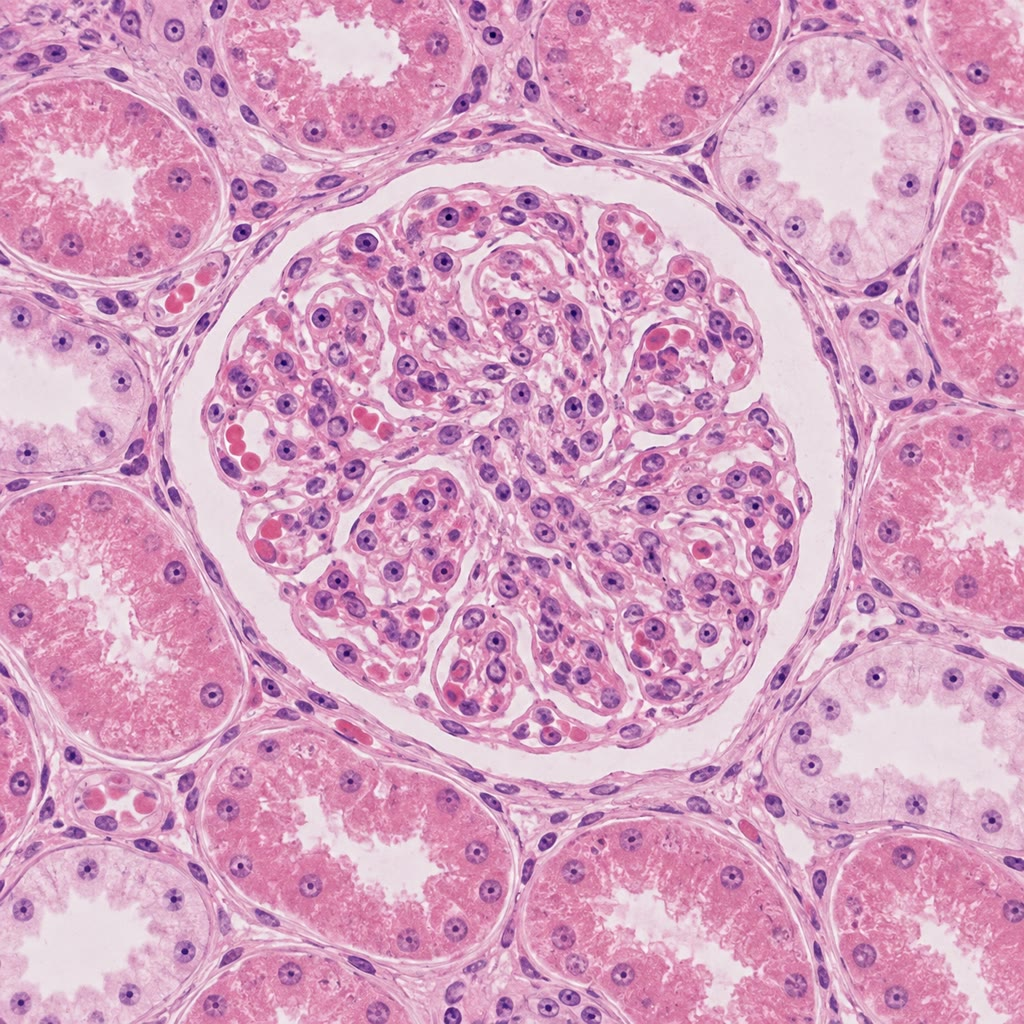
\includegraphics[width=0.46\linewidth]{images/book5/ai/b5-20-kidney-section.jpg}\hspace{0.04\linewidth}
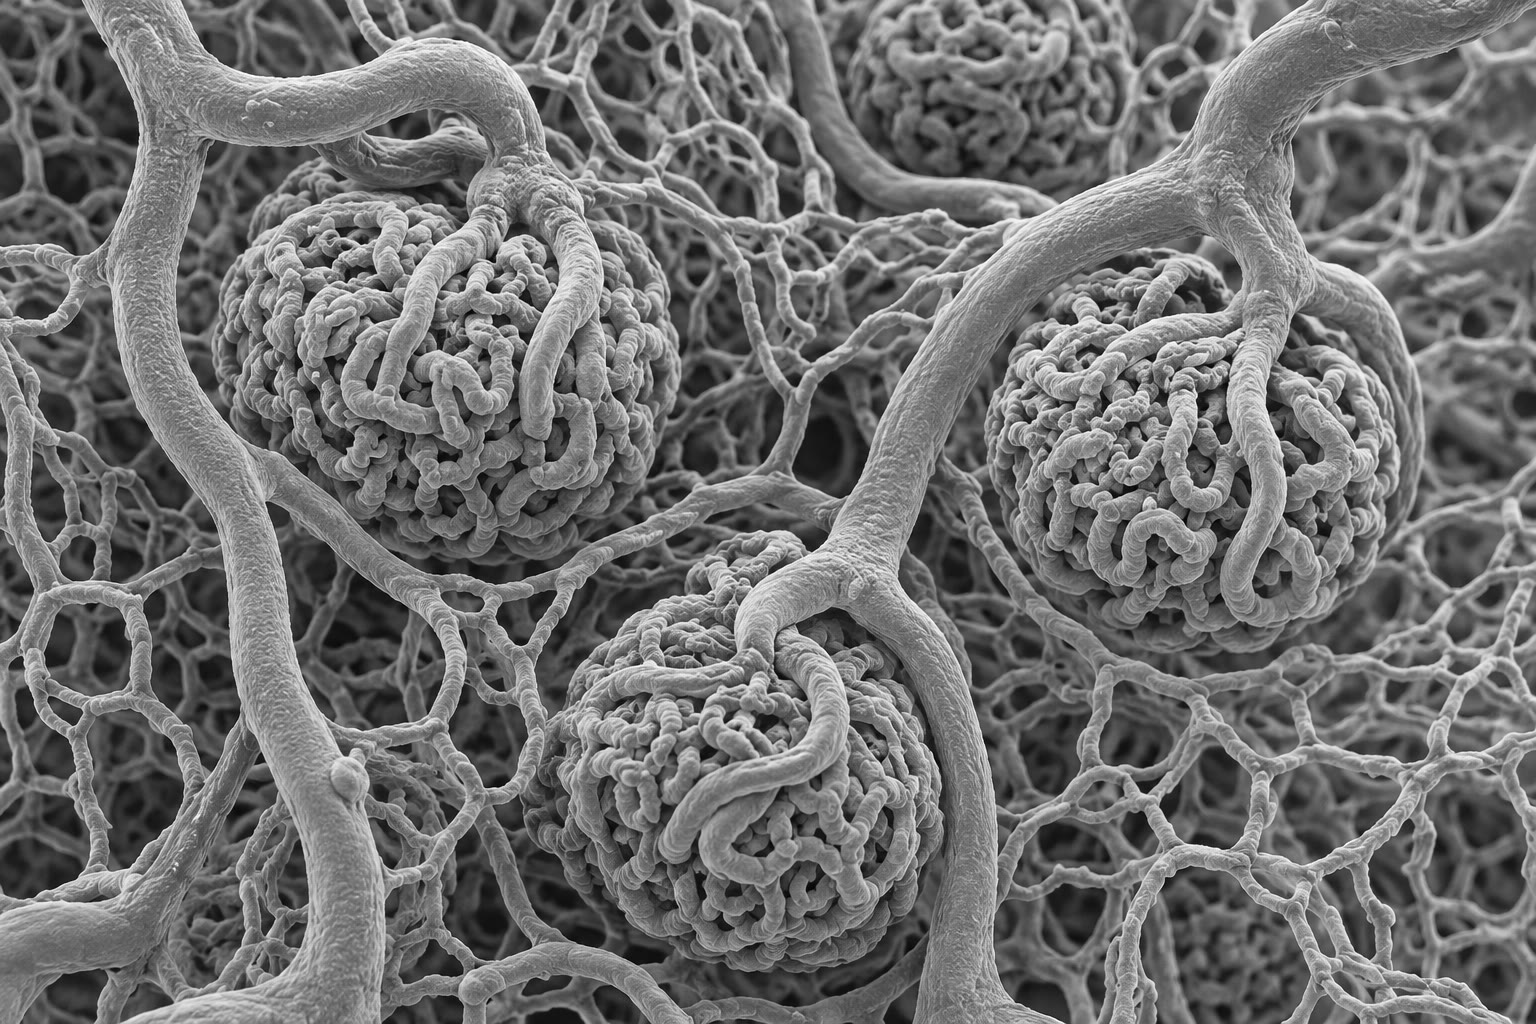
\includegraphics[width=0.46\linewidth]{images/book5/ai/b5-20-nephron-cast.jpg}

{\small À gauche~: le cortex rénal en coupe --- un \omterm{def:b3:renal-osmoregulation:nephron}{glomérule} dans sa
capsule parmi les profils de tubes proximaux et distaux. À droite~: un
moulage vasculaire du cortex, chaque pelote de laine un \omterm{def:b3:renal-osmoregulation:nephron}{glomérule} avec
ses vaisseaux afférent et efférent parmi les capillaires
péritubulaires.}
\end{omfigure}

\section{D'autres animaux, d'autres solutions}

\begin{definition}[L'osmorégulation à travers le règne animal]\label{def:b3:renal-osmoregulation:comparative}
\index{tube de Malpighi}\index{glande à sel}\index{cellule à chlorure}\index{eau métabolique}\index{épaisseur médullaire relative}
Les poissons d'eau douce vivent dans un milieu dix fois moins osmolaire
que leur sang~: l'eau afflue par les branchies, le sel fuit, et ils
excrètent une urine abondante et diluée et captent activement le sel par
les \emph{cellules à chlorure} de leurs branchies, sans jamais boire.
Les téléostéens marins, dont le sang vaut le tiers de l'\omterm{def:b3:renal-osmoregulation:problem}{osmolarité} de la
mer, perdent de l'eau par les branchies, boivent l'eau de mer et
rejettent le sel par les mêmes cellules à chlorure fonctionnant à
l'envers, en gardant une urine chiche~; les requins, eux, tiennent leur
sang iso-osmotique à la mer en retenant de l'urée (et de l'oxyde de
triméthylamine pour stabiliser leurs protéines contre elle), et
excrètent le sel en excès par une glande rectale. Les oiseaux marins et
les reptiles marins portent au-dessus des yeux des \emph{glandes à sel}
qui sécrètent une saumure deux fois plus salée que la mer, ce qui permet
à un albatros de boire à l'océan. Les insectes filtrent par des
\emph{tubes de Malpighi} mus par une sécrétion active de potassium
plutôt que par la pression sanguine, et réabsorbent l'eau dans le rectum
si complètement que les crottes d'un ténébrion du désert sont sèches.
Chez les mammifères le pouvoir de concentration suit la longueur des
anses rapportée à la taille du rein (l'\emph{épaisseur médullaire
relative})~: un castor atteint \qty{500}{mOsm/L}, un humain \num{1200},
un chameau \num{3000}, le rat kangourou \num{5500} --- ce qui lui permet
de vivre de l'\emph{eau métabolique} libérée par l'oxydation de sa
nourriture, environ \qty{0.6}{g} d'eau par gramme d'amidon, avec un nez
qui récupère l'eau de chaque expiration par refroidissement à
contre-courant.
\end{definition}

\begin{omfigure}
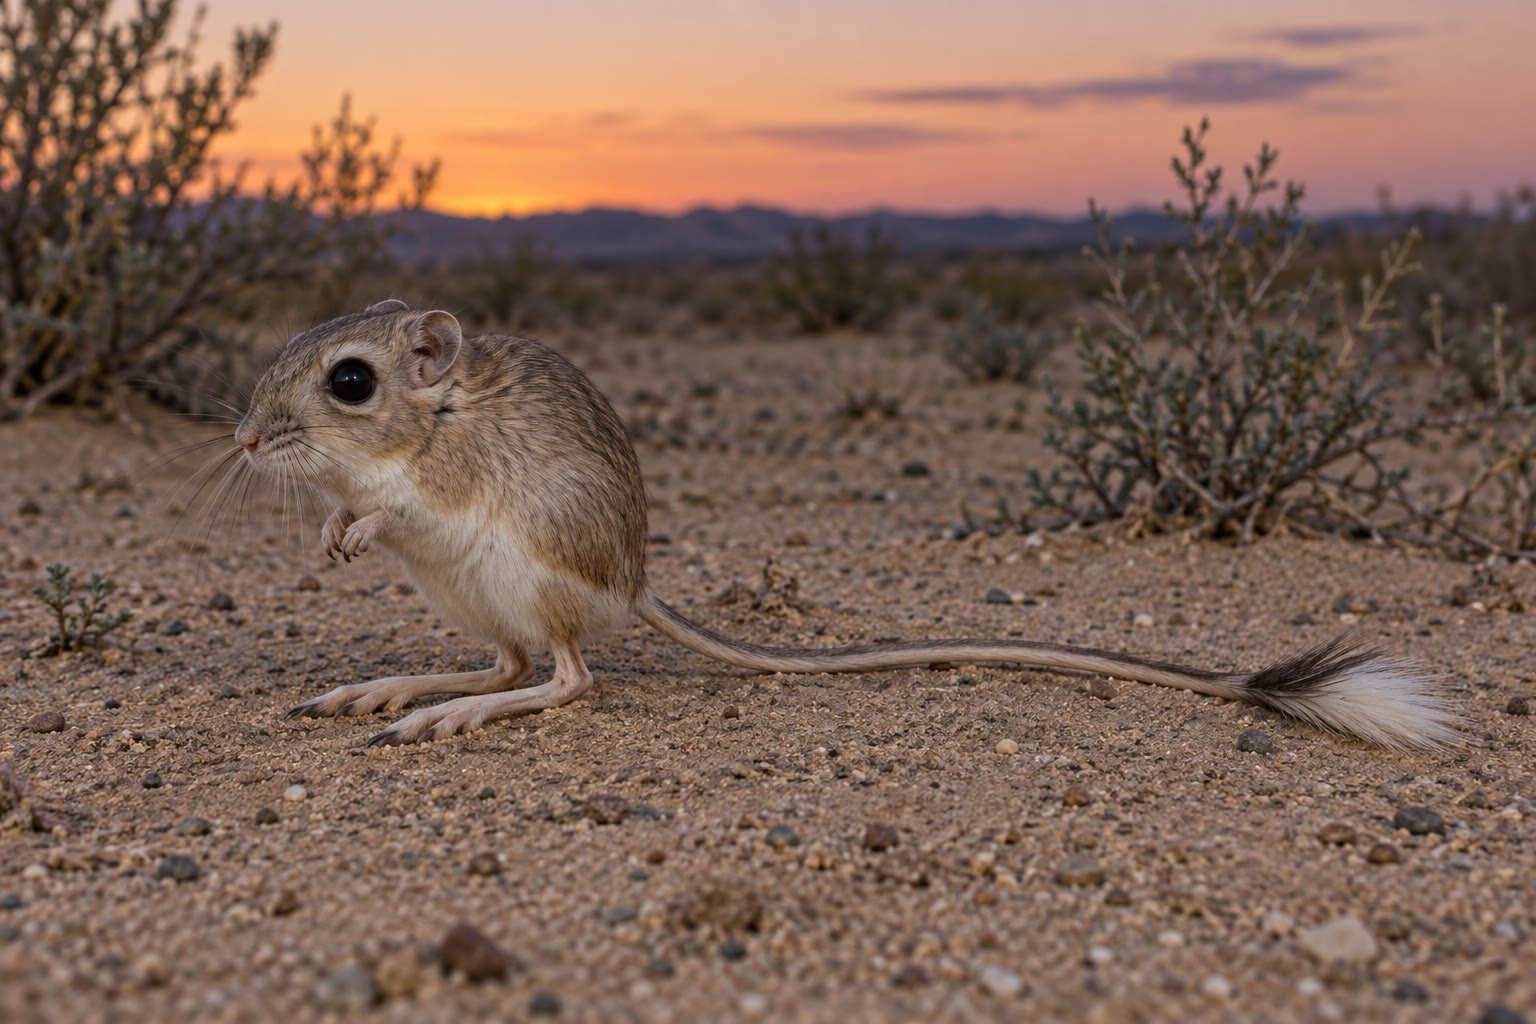
\includegraphics[width=0.56\linewidth]{images/book5/ai/b5-20-kangaroo-rat.jpg}

{\small Un rat kangourou, qui ne boit jamais~: de longues \omterm{def:b3:renal-osmoregulation:nephron}{anses de
Henle}, une urine cinq fois plus concentrée que l'eau de mer, un nez
froid qui condense l'eau de chaque souffle, et un régime dont
l'oxydation fait toute l'eau dont il a besoin.}
\end{omfigure}

\begin{remark}[Le rein comme problème de conception]\label{rem:b3:renal-osmoregulation:design}
Le rein des mammifères filtre quarante fois le volume plasmatique par
jour pour en reprendre presque tout~: conception extravagante, dont le
propos est que tout filtrer et réabsorber sélectivement est plus simple
que sécréter sélectivement chaque déchet susceptible d'apparaître. Son
coût est les \qty{7}{\%} du métabolisme de repos dépensés à repomper le
sodium, et sa vulnérabilité est le filtre délicat, qui lâche lentement
sous une pression élevée et un glucose élevé. Son astuce est l'anse à
contre-courant, dispositif qu'on retrouve dans les vessies natatoires
des poissons profonds, les pattes des échassiers et le nez des rongeurs
du désert, par lequel une petite différence locale, qu'on peut se payer,
s'empile en une grande --- la même idée, chaque fois~: qu'un gradient
peut se bâtir à partir d'un écoulement.
\end{remark}

\section{Exercices}

\begin{exercise}[$\star$]\label{exo:b3:renal-osmoregulation:1}
Nommer dans l'ordre les segments du \omterm{def:b3:renal-osmoregulation:nephron}{néphron} et dire une chose que fait
chacun.
\end{exercise}

\begin{exercise}[$\star$]\label{exo:b3:renal-osmoregulation:2}
Définir la clairance. Une substance a une concentration plasmatique de
\qty{2}{mg/mL}, une concentration urinaire de \qty{100}{mg/mL} et le
débit urinaire vaut \qty{1.5}{mL/min}. Calculer sa clairance et dire si
elle est réabsorbée, sécrétée ou ni l'un ni l'autre, si le DFG vaut
\qty{120}{mL/min}.
\end{exercise}

\begin{exercise}[$\star$]\label{exo:b3:renal-osmoregulation:3}
Pourquoi un poisson d'eau douce ne boit-il jamais et un poisson marin
sans cesse~? Que font les branchies dans chaque cas~?
\end{exercise}

\begin{exercise}[$\star$]\label{exo:b3:renal-osmoregulation:4}
Qu'est-ce que l'\omterm{prop:b3:renal-osmoregulation:countercurrent}{effet unitaire} de l'\omterm{def:b3:renal-osmoregulation:nephron}{anse de Henle}, quelle branche le
produit, et pourquoi les deux branches doivent-elles différer par leur
perméabilité à l'eau~?
\end{exercise}

\begin{exercise}[$\star\star$]\label{exo:b3:renal-osmoregulation:5}
Pression capillaire glomérulaire \qty{60}{mmHg}, espace de Bowman
\qty{18}{mmHg}, pression oncotique plasmatique \qty{28}{mmHg} à
l'extrémité afférente montant à \qty{35}{mmHg} à l'extrémité efférente.
Calculer la pression nette de filtration à chaque extrémité et
expliquer pourquoi la filtration peut cesser avant la fin du capillaire.
Qu'en déduire sur l'effet du débit plasmatique sur le DFG~?
\end{exercise}

\begin{exercise}[$\star\star$]\label{exo:b3:renal-osmoregulation:6}
La clairance de la créatinine d'un patient vaut \qty{40}{mL/min}. Le
sodium plasmatique vaut \qty{140}{mmol/L}, le sodium urinaire
\qty{70}{mmol/L}, le débit urinaire \qty{1}{mL/min}. Calculer la charge
filtrée de sodium, l'excrétion, la fraction réabsorbée et la clairance
du sodium.
\end{exercise}

\begin{exercise}[$\star\star$]\label{exo:b3:renal-osmoregulation:7}
Une personne suit un régime qui produit \qty{900}{mOsm} de soluté par
jour et sait concentrer jusqu'à \qty{1200}{mOsm/L}. Volume urinaire
minimal~? Si une maladie rénale abaisse le maximum à \qty{400}{mOsm/L},
combien doit-elle boire pour rester en équilibre, en comptant
\qty{0.9}{L} de perte insensible~?
\end{exercise}

\begin{exercise}[$\star\star$]\label{exo:b3:renal-osmoregulation:8}
Prévoir le volume et l'\omterm{def:b3:renal-osmoregulation:problem}{osmolarité} de l'urine, le sodium plasmatique et
l'état de la soif dans (a) un diabète insipide, (b) une sécrétion
inappropriée de vasopressine par une \omterm{def:b3:cancer-biology:hallmarks}{tumeur}, (c) un excès
d'\omterm{def:b3:renal-osmoregulation:controls}{aldostérone}, (d) un régime sans sel pendant une semaine.
\end{exercise}

\begin{exercise}[$\star\star$]\label{exo:b3:renal-osmoregulation:9}
Calculer la \omterm{prop:b3:renal-osmoregulation:water}{clairance de l'eau libre} pour une urine à \qty{100}{mOsm/L}
à \qty{6}{mL/min} et pour une urine à \qty{1000}{mOsm/L} à
\qty{0.6}{mL/min}, le plasma étant à \qty{300}{mOsm/L}. Interpréter
chacune.
\end{exercise}

\begin{exercise}[$\star\star\star$]\label{exo:b3:renal-osmoregulation:10}
Modéliser l'anse en $n$ étages où le liquide ascendant de chaque étage
est \qty{200}{mOsm/L} au-dessous de l'interstitium et le liquide
descendant lui est égal, le liquide entrant à \qty{300}{mOsm/L}.
Argumenter que l'\omterm{def:b3:renal-osmoregulation:problem}{osmolarité} stationnaire au coude peut approcher $300 +
200n$, de sorte que le gradient est limité par la longueur de l'anse et
par l'\omterm{prop:b3:renal-osmoregulation:countercurrent}{effet unitaire} de la pompe, et dire ce qui fixe physiquement $n$.
\end{exercise}

\begin{exercise}[$\star\star\star$]\label{exo:b3:renal-osmoregulation:11}
Un rat kangourou mange \qty{5}{g} de graines sèches par jour,
\qty{80}{\%} d'amidon, oxydé en CO$_{2}$ et en eau (\qty{0.6}{g} d'eau
par gramme d'amidon). Il doit excréter \qty{3}{mOsm} de soluté par jour
à \qty{5500}{mOsm/L}, et perd \qty{1.5}{g} d'eau par jour par
évaporation depuis un nez qui récupère \qty{70}{\%} de l'eau de son
souffle. Faire le bilan de son eau et dire s'il survit sans boire.
\end{exercise}

\begin{exercise}[$\star\star\star$]\label{exo:b3:renal-osmoregulation:12}
La dialyse fait passer le sang d'un côté d'une membrane et le dialysat
de l'autre, à contre-courant. Expliquer pourquoi un écoulement à
contre-courant épure plus qu'un écoulement parallèle, estimer la
clairance d'une machine qui retire l'urée de \qty{300}{mL/min} de sang
avec \qty{70}{\%} d'efficacité, et comparer à deux reins sur une semaine
si la machine tourne quatre heures trois fois par semaine.
\end{exercise}

\section{Problème~: dix-huit seaux par jour}

\begin{problem}[{Problème du week-end --- le filtrat d'une journée suivi
du glomérule à la vessie~: les pressions de Starling, les clairances de
quatre substances, le seuil du glucose, le bilan de l'eau de la dilution
maximale à l'eau de mer, et l'équilibre d'un rongeur du désert, pour
finir sur le DFG, le volume urinaire obligatoire et l'eau nette que
rapporte un litre d'eau de mer}]
\label{pb:b3:renal-osmoregulation:1}
Données~: $K_{f} = \qty{12.5}{mL/min/mmHg}$~; $P_{\text{CG}} = \qty{55}{mmHg}$,
$P_{\text{EB}} = \qty{15}{mmHg}$, $\pi_{\text{CG}} = \qty{30}{mmHg}$.
Plasma~: inuline \qty{0.5}{mg/mL}, créatinine \qty{0.01}{mg/mL}, urée
\qty{5}{mmol/L}, glucose \qty{5}{mmol/L}, acide para-aminohippurique
\qty{0.02}{mg/mL}, Na$^{+}$ \qty{140}{mmol/L}, \omterm{def:b3:renal-osmoregulation:problem}{osmolarité}
\qty{290}{mOsm/L}. Débit urinaire \qty{1}{mL/min}~: inuline \qty{62.5}{mg/mL},
créatinine \qty{1.3}{mg/mL}, urée \qty{250}{mmol/L}, glucose $0$,
acide para-aminohippurique \qty{13}{mg/mL}, Na$^{+}$ \qty{100}{mmol/L},
\omterm{def:b3:renal-osmoregulation:problem}{osmolarité} \qty{600}{mOsm/L}. Hématocrite $0.45$. Glucose $T_{m} =
\qty{375}{mg/min}$ (\qty{2.1}{mmol/min}). Soluté quotidien \qty{600}{mOsm}~;
$U_{\max} = \qty{1200}{mOsm/L}$, $U_{\min} = \qty{50}{mOsm/L}$~;
perte insensible \qty{0.9}{L/d}~; eau de mer \qty{1000}{mOsm/L}.

\medskip
\noindent\textbf{Partie I --- Le filtre.}
\begin{enumerate}
  \item Calculer la pression nette de filtration et le DFG.
  \item Convertir le DFG en litres par jour. Combien de fois le volume
        plasmatique (\qty{3}{L}) est-il filtré~?
  \item Calculer la clairance de l'inuline et la comparer au DFG.
        Calculer la clairance de la créatinine~; pourquoi est-elle un
        peu plus grande~?
  \item Calculer la clairance de l'acide para-aminohippurique (le débit
        plasmatique rénal), le débit sanguin rénal et la fraction de
        filtration.
  \item L'artériole efférente se resserre et porte $P_{\text{CG}}$ à
        \qty{60}{mmHg}. Nouveau DFG~? Pourquoi les médicaments qui
        bloquent l'angiotensine~II abaissent-ils un peu le DFG d'un rein
        sain et protègent-ils celui d'un diabétique~?
  \item Des protéines apparaissent dans l'urine à \qty{3}{g/d}. Quelle
        couche du filtre a lâché, et qu'advient-il de la pression
        oncotique plasmatique et des tissus si cela continue~?
\end{enumerate}

\medskip
\noindent\textbf{Partie II --- Le traitement.}
\begin{enumerate}[resume]
  \item L'urée~: charge filtrée, excrétion, fraction réabsorbée et
        clairance.
  \item Le sodium~: charge filtrée par jour en moles et en grammes,
        excrétion, et fraction réabsorbée. Combien de kilogrammes de sel
        seraient perdus en un jour si rien n'était réabsorbé~?
  \item Le glucose~: charge filtrée en mmol/min et en grammes par jour~;
        en excrète-t-on~? À quelle glycémie la charge filtrée
        atteint-elle $T_{m}$ (le seuil)~?
  \item Un diabétique a une glycémie de \qty{20}{mmol/L}. Glucose
        excrété par minute et par jour en grammes, et volume urinaire
        supplémentaire si chaque \qty{300}{mOsm} de glucose emporte
        \qty{1}{L} à la concentration qui règne. Expliquer la soif et
        l'amaigrissement du diabète non traité.
  \item Réabsorber le sodium coûte un ATP pour trois Na$^{+}$. Combien
        de moles d'ATP par jour le rein dépense-t-il pour le sodium, et
        combien de kilojoules (\qty{50}{kJ/mol})~? Comparer à un
        métabolisme de repos de \qty{7}{MJ/d}.
  \item Expliquer pourquoi le rein filtre et réabsorbe plutôt que de
        sécréter chaque déchet, en termes de ce que le tube devrait
        savoir reconnaître.
\end{enumerate}

\medskip
\noindent\textbf{Partie III --- L'eau.}
\begin{enumerate}[resume]
  \item Clairance osmolaire $U_{\text{osm}}V/P_{\text{osm}}$ d'après les
        données, et \omterm{prop:b3:renal-osmoregulation:water}{clairance de l'eau libre}. La personne conserve-t-elle
        ou perd-elle de l'eau~?
  \item Volume urinaire minimal pour le soluté quotidien~; maximal (à
        $U_{\min}$)~; le besoin quotidien total en eau au minimum, avec
        la perte insensible.
  \item On boit un litre d'eau de mer. Combien d'urine faut-il pour en
        excréter le sel à $U_{\max}$, et quel est le gain net en eau
        avant que le soluté propre à la journée soit compté~? Et après~?
  \item La vasopressine est absente (diabète insipide) et l'urine reste
        à $U_{\min}$. Volume urinaire quotidien pour le même soluté, et
        eau qu'il faut boire chaque jour pour tenir l'équilibre.
  \item De la bière à \qty{20}{mOsm/L}~: combien peut-on en boire par
        jour avant que le rein, à $U_{\min}$, ne puisse plus excréter
        l'eau~? (L'eau en excès de ce que le soluté peut emporter à
        $U_{\min}$ s'accumule.)
  \item Après une nuit sans eau l'\omterm{def:b3:renal-osmoregulation:problem}{osmolarité} plasmatique vaut
        \qty{298}{mOsm/L}. De combien de pour cent a-t-elle monté, et
        que fait l'hypothalamus~? Estimer le déficit en eau si l'eau
        corporelle totale vaut \qty{42}{L} et que le soluté est
        inchangé.
  \item Expliquer pourquoi un coureur de marathon qui boit \qty{6}{L}
        d'eau tout en perdant du sel par la sueur peut voir son sodium
        plasmatique tomber dangereusement bas, et ce que le rein devrait
        faire pour l'empêcher.
\end{enumerate}

\medskip
\noindent\textbf{Partie IV --- Le désert.}
\begin{enumerate}[resume]
  \item Un rat kangourou excrète \qty{3}{mOsm} par jour à \qty{5500}{mOsm/L}.
        Volume urinaire~? Comparer au volume dont un rein humain aurait
        besoin pour le même soluté à son propre maximum.
  \item Sa nourriture donne \qty{2.4}{g} d'\omterm{def:b3:renal-osmoregulation:comparative}{eau métabolique} par jour et
        il perd \qty{1.6}{g} en respirant et \qty{0.3}{g} dans ses
        fèces. Faire le bilan avec l'urine de la question 20.
  \item Un chameau concentre jusqu'à \qty{3000}{mOsm/L} et tolère de
        perdre \qty{25}{\%} de son eau corporelle. Pour un chameau de
        \qty{500}{kg} à \qty{65}{\%} d'eau, combien peut-il perdre, et
        combien de jours cela couvre-t-il à raison de \qty{5}{L/d}~?
  \item Un oiseau marin mange \qty{200}{g} de poisson et boit
        \qty{100}{mL} d'eau de mer par jour, ce qui lui apporte
        \qty{150}{mmol} de NaCl. Sa \omterm{def:b3:renal-osmoregulation:comparative}{glande à sel} sécrète à
        \qty{800}{mmol/L}. Combien de saumure produit-il, et pourquoi la
        glande vaut-elle mieux que le rein (qui, chez les oiseaux, ne
        concentre qu'à \qty{600}{mOsm/L}) pour cela~?
  \item Un poisson d'eau douce de \qty{100}{g} gagne par ses branchies
        \qty{30}{\%} de sa masse corporelle en eau par jour. Combien
        d'urine doit-il faire, à quelle \omterm{def:b3:renal-osmoregulation:problem}{osmolarité} par rapport à son
        sang, et qu'adviendrait-il de son sel sans capture active~?
  \item Résumer~: le DFG (question~1), le volume urinaire obligatoire
        (question~14), et l'eau nette d'un litre d'eau de mer une fois
        compté le soluté de la journée (question~15).
\end{enumerate}
\end{problem}
